\documentclass[11pt,letterpaper]{article}
\usepackage[lmargin=1in,rmargin=1in,tmargin=1in,bmargin=1in]{geometry}
\usepackage{../style/homework}
\usepackage{../style/commands}
\setbool{quotetype}{true} % True: Side; False: Under
\setbool{hideans}{true} % Student: True; Instructor: False

% -------------------
% Content
% -------------------
\begin{document}

\homework{1: Due 09/14}{I can be just as non-competitive as anybody. Matter of fact, I'm the most non-competitive, so I win.}{Peter Griffin, Family Guy}

% Problem 1
\problem{10} Showing all the steps according to order of operations, compute the following:
	\begin{enumerate}[(a)]
	\item $10 + 10 - 16 \cdot 0 + 2 + 2$
	\item $(-1)^3 - 1 + 4^2/2$
	\item $15 - (6 - 10) + 3^2$
	\item $\dfrac{-4 - (2 - 4)^2}{3^2 - 1}$
	\end{enumerate}



\newpage



% Problem 2
\problem{10} Define the following sets:
	\[
	\begin{aligned}
	A&= \{ 1,\; 2, \; 3,\; 4,\; 5,\; 6,\; 7,\; 8,\; 9,\; 10 \} \\
	B&= \{ 2,\; 4,\; 6,\; 8,\; 10 \} \\
	C&= \{ 1,\; 3,\; 5,\; 7,\; 9 \} \\
	D&= \{ 2,\; 3,\; 5,\; 7 \}
	E&= \{ 2,\; 3,\; 4,\; 6,\; 8,\; 9 \}
	\end{aligned}
	\]
Consider all these sets as subsets of $A$. Compute the following:
	\begin{enumerate}[(a)]
	\item $B^c$
	\item $B \cup D$
	\item $E \setminus D$
	\item $C \cap E$
	\item $|A|$
	\end{enumerate}



\newpage



% Problem 3
\problem{10} Define the following sets:
	\[
	\begin{aligned}
	A&= \text{All males over 40~years old.} \\ 
	B&= \text{All people that have acted in a movie.} \\
	C&= \text{All US Presidents, alive or dead.} \\
	D&= \text{All persons under 6~ft tall.} 
	\end{aligned}
	\]
Consider all of these sets as subsets of the set of all people alive. Being sure to completely justify your response, answer the following:
	\begin{enumerate}[(a)]
	\item Find an element of $A \cap B$. 
	\item Is Jeff Bezos~$\in A \cup C$? Is Jeff Bezos~$\in C \cup D$?
	\item Is George Washington$\in C - B$?
	\item Is Danny Devito~$\in D^C$?
	\item Are sets $B$ and $C$ disjoint? [Hint: Consider US~Presidents from the last 50~years.]
	\end{enumerate}



\newpage




% Problem 4
\problem{10} Determine whether the following relations are functions, being sure to justify your answer. If the relation is a function, determine its domain, codomain, and range. [For this problem, in determining a functions domain, codomain, and range, you may invoke the use/description of a graph.]
	\begin{enumerate}[(a)]
	\item \phantom{.}\par
	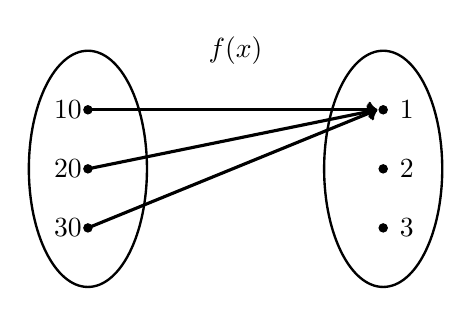
\begin{tikzpicture}[scale=0.75]
	\node at (2.5,2) {$f(x)$};
	% Ellipses
	\draw[line width=0.03cm] (0,0) circle (1 and 2);
	\draw[line width=0.03cm] (5,0) circle (1 and 2);
	
	% Nodes
	\draw[fill=black] (0,1) circle (0.07);
	\draw[fill=black] (0,0) circle (0.07);
	\draw[fill=black] (0,-1) circle (0.07);
	
	\draw[fill=black] (5,1) circle (0.07);
	\draw[fill=black] (5,0) circle (0.07);
	\draw[fill=black] (5,-1) circle (0.07);
	
	% Arrow
	\draw[line width=0.04cm,->] (0,1) -- (4.9,1);
	\draw[line width=0.04cm,->] (0,0) -- (4.9,1);
	\draw[line width=0.04cm,->] (0,-1) -- (4.9,1);
	
	% Labels
	\node at (-0.3,1) {$10\,$};
	\node at (-0.3,0) {$20\,$};
	\node at (-0.3,-1) {$30\,$};
	
	\node at (5.4,1) {$1$};
	\node at (5.4,0) {$2$};
	\node at (5.4,-1) {$3$};
	\end{tikzpicture}

	\item \phantom{.}\par
	\hspace{1cm}\begin{table}[!ht]
	\setlength\arrayrulewidth{0.02cm}
	\begin{tabular}{cc|r}
	\hspace{1cm} & $x$ & $g(x)$ \\ \cline{2-3} 
	& $1.0$ & $1.0$ \\
	& $1.5$ & $4.3$ \\
	& $3.0$ & $-6.1$ \\
	& $4.4$ & $2.2$ \\
	& $6.8$ & $1.0$ 
	\end{tabular}
	\end{table}
	
	\item $h(x, y)= x + y^4$. 
	
	\item $j(x)=$ the multiple of two closest to $x$.
	\end{enumerate}



\newpage



% Problem 5
\problem{10} Suppose that $f(x, y)$ is the function given by the following table:
	\begin{table}[!ht]
	\centering
	\begin{tabular}{|c||r|r|r|r|} \hline 
	$x \backslash y$ & $1$ & $2$ & $3$ & $4$ \\ \hline \hline
	$1$ & $-2$ & $7$ & $4$ & $-4$ \\ \hline
	$2$ & $0$ & $3$ & $-1$ & $1$ \\ \hline
	$3$ & $5$ & $-6$ & $7$ & $6$ \\ \hline
	$4$ & $1$ & $0$ & $4$ & $0$ \\ \hline
	\end{tabular}
	\end{table} \par
Showing all your work, compute the following:
	\begin{enumerate}[(a)]
	\item $f(3, 2)$
	\item $f(3 - 1, 2^2)$
	\item $5 f(3, 1) - 8$
	\item $\dfrac{4 - f\big( 3^2 + (-2)^3, 1 \big) }{2 f(1, 3)}$
	\end{enumerate}



\newpage



% Problem 6
\problem{10} Let $\text{rdwn}(x)$ denote the largest integer that is {\itshape less than} $x$. 
	\begin{enumerate}[(a)]
	\item Find $\text{rdwn}(x)$ for $x= 0.5, 2.2, 5.9, 6.0, -1.5, -4.9, -7$. 
	\item Explain why $\text{rdwn}(x)$ is a function.
	\item Being as accurate as possible, sketch a graph of $\text{rdwn}(x)$ on the plot below. 
	\[
	\fbox{%
	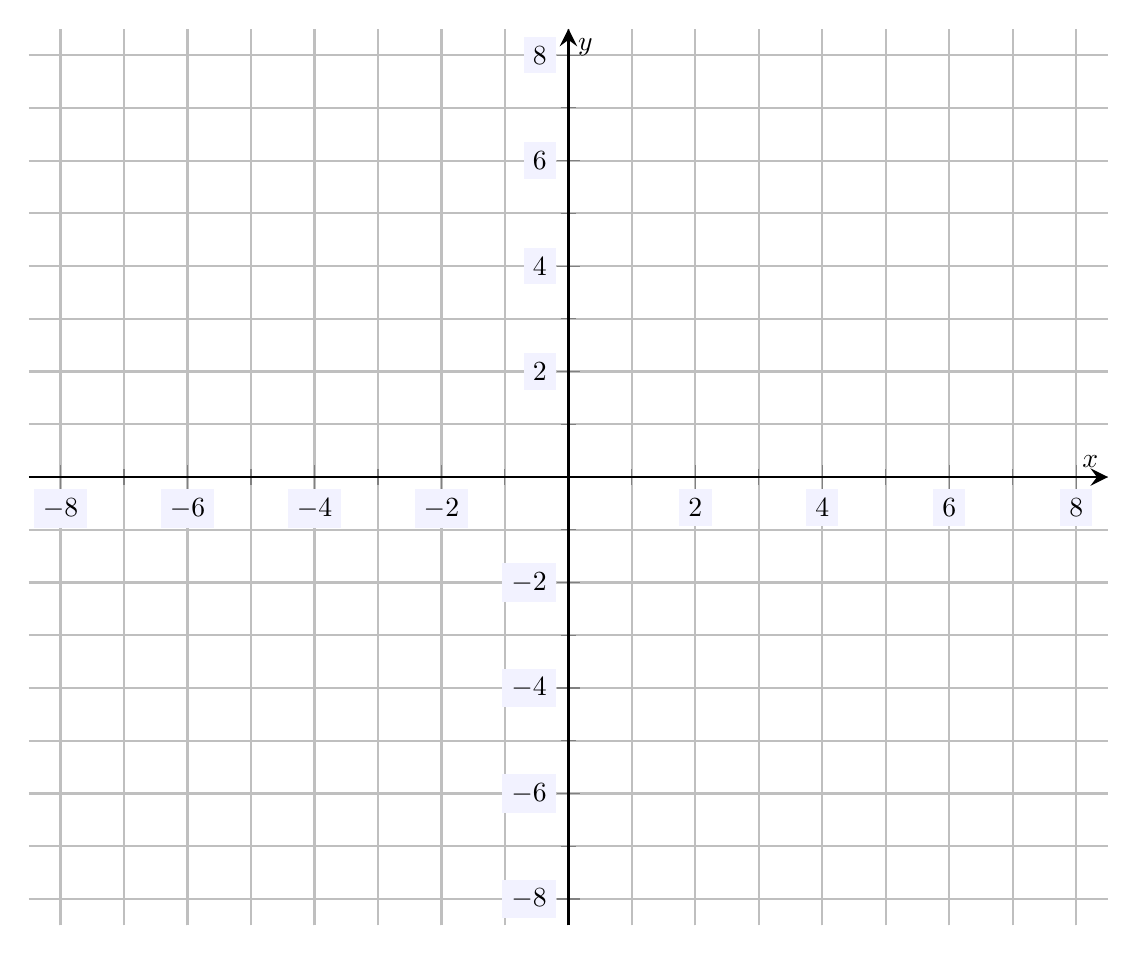
\begin{tikzpicture}[scale=2,every node/.style={scale=0.5}]
	\begin{axis}[
	grid=both,
	axis lines=middle,
	ticklabel style={fill=blue!5!white},
	xmin= -8.5, xmax=8.5,
	ymin= -8.5, ymax=8.5,
	xtick={-8,-6,-4,-2,0,2,4,6,8},
	ytick={-8,-6,-4,-2,0,2,4,6,8},
	minor tick = {-8,-7,...,8},
	xlabel=\(x\),ylabel=\(y\),
	]
	\end{axis}
	\end{tikzpicture}
	}
	\]
	\end{enumerate}


\end{document}